\chapter[Using a Facade Pattern to combine Computer Vision Services]
{Using a Facade Pattern to combine Computer Vision Services\pubfootnote{Ohtake:2019vi}}
\label{ch:icwe2019}
\graphicspath{{mainmatter/publications/figures/icwe2019/}}

\glsresetall
\begin{abstract}
Intelligent \glslongpl{cvs}, such as Google Cloud Vision or Amazon Rekognition, are becoming evermore pervasive and easily accessible to developers to build applications.
Because of the stochastic nature that \glsac{ml} entails and disparate datasets used in their training, the outputs from different computer vision services varies with time, resulting in low reliability---for some cases---when compared against each other.
Merging multiple unreliable \glsac{api} responses from multiple vendors may increase the reliability of the overall response, and thus the reliability of the intelligent end-product.
We introduce a novel methodology---inspired by the proportional representation used in electoral systems---to merge outputs of different intelligent computer vision \glsac{api} provided by multiple vendors.
Experiments show that our method outperforms both naive merge methods and traditional proportional representation methods by 0.015 F-measure.
\end{abstract}
\glsresetall

\section{Introduction}

With the introduction of \glspl{iws} that make \gls{ml} more accessible to developers \citep{Ribeiro:2015dz,Hwang:2017tr}, we have seen a large growth of intelligent applications dependent on such services \citep{Mapillar97:online,FileShad33:online}.
For example, consider the advances made in computer vision, where objects are localised within an image and labelled with associated categories.
Cloud-based \glspl{cvs}---e.g., \citepweb{GoogleCloud:Home,Azure:Home,AWS:Home,IBM:Home,Clarifai:Home,DeepAI:Home,Imagaa:Home,Talkwaler:Home}---are a subset of \glspl{iws}. They utilise \gls{ml} techniques to achieve image recognition via a remote black-box approach, thereby reducing the overhead for application developers to understand how to implement intelligent systems from scratch. Furthermore, as the processing and training of the machine-learnt algorithms is offloaded to the cloud, developers simply send \glsac{rest}ful \glsac{api} requests to do the recognition. There are, however, inherit differences and drawbacks between traditional \glslongpl{ws} and \glspl{iws}, which we describe with the motivating scenario below.

\subsection{Motivating Scenario: Intelligent vs Traditional Web Services}

An application developer, Tom, wishes to develop a social media Android and iOS app that catalogues photos of him and his friends, common objects in the photo, and generates brief descriptions in the photo (e.g., all photos with his husky dog, all photos on a sunny day etc.). Tom comes from a typical software engineering background with little knowledge of computer vision and its underlying concepts. He knows that intelligent computer vision web \glsacpl{api} are far more accessible than building a computer vision engine from scratch, and opts for building his app using these cloud services instead.

Based on his experiences using similar cloud services, Tom would expect consistency of the results from the same \glsac{api} and different \glsacpl{api} that provide the same (or similar) functionality. As an analogy, when Tom writes the Java substring method \texttt{"doggy".substring(0, 2)}, he expects it to be the same result as the Swift equivalent \texttt{"doggy".prefix(3)}. Each and every time he interacts with the substring method using either \glsac{api}, he gets \texttt{"dog"} as the response. This is because Tom is used to deterministic, rule-driven \glsacpl{api} that drive the implementation behind the substring method.

Tom's deterministic mindset results in three key differentials between a traditional \glslong{ws} and an \gls{iws}:
\begin{enumerate}[label=\textbf{(\arabic*)}]
    \item \textbf{Given similar input, results differ between similar \glspl{iws}.}
    When Tom interacts with the \glsac{api} of an \gls{iws}, he is not aware that each \glsac{api} provider trains their own, unique \gls{ml} model, both with disparate methods and datasets. These \glspl{iws} are, therefore, nondeterministic and data-driven; input images---even if they contain the same conceptual objects---often output different results. Contrast this to the substring method of traditional \glsacpl{api}; regardless of what programming language or string library is used, the same response is expected by developers.
    \item \textbf{Intelligent responses are not certain.}
    When Tom interprets the response object of an \gls{iws}, he finds that there is a `confidence' value or `score'. This is because the \gls{ml} models that power \glspl{iws} are inherently probabilistic and stochastic; any insight they produce is purely statistical and associational~\citep{Pearl:2018uv}. Unlike the substring example, where the rule-driven implementation provides certainty to the results, this is not guaranteed for \glspl{iws}.
    For example, a picture of a husky breed of dog is misclassified as a wolf. This could be due to adversarial examples \citep{Szegedy:2013vw} that `trick' the model into misclassifying images when they are fully decipherable to humans. It is well-studied that such adversarial examples exist in the real world unintentionally \citep{Kurakin:2016vw,Eykholt:2018vk,Pezzementi:2018tq}.
    \item \textbf{Intelligent \glsacpl{api} evolve over time.}
    Tom may find that responses to processing an image may change over time; the labels he processes in testing may evolve and therefore differ to when in production. In traditional \glslongpl{ws}, evolution in responses is slower, generally well-communicated, and usually rare (Tom would always expect \texttt{"dog"} to be returned in the substring example). This has many implications on software systems that depend on these \glsacpl{api}, such as confidence in the output and portability of the solution. Currently, if Tom switches from one \glsac{api} provider to another, or if he doesn't regularly test his app in production, he may begin to see a very different set of labels and confidence levels.
\end{enumerate}

\subsection{Research Motivation}

These drawbacks bring difficulties to the intended \glsac{api} users like Tom. We identify a gap in the software engineering literature regarding such drawbacks, including: lack of best practices in using \glspl{iws}; assessing and improving the reliability of \glsacpl{api} for their use in end-products; evaluating which \glsac{api} is suitable for different developer and application needs; and how to mitigate risk associated with these \glsacpl{api}. We focus on improving reliability of \glspl{cvs} for use in end-products.
The key research questions in this paper are:
\begin{enumerate}[label=\textbf{RQ\arabic*:},leftmargin=3\parindent]
  \item Is it possible to improve reliability by merging multiple \gls{cvs} results?
  \item Are there better algorithms for merging these results than currently in use?
\end{enumerate}

Previous attempts at overcoming low reliability include triple-modular redundancy \citep{IBMTripleModularRedendancy}.
This method uses three modules and decides output using majority rule.
However, in \glspl{cvs}, it is difficult to apply majority rule: these \glsacpl{api} respond with a list of labels and corresponding scores.
Moreover, disparate \glsacpl{api} ordinarily output different results. These differences make it hard to apply majority rule because the type of outputs are complex and disparate \glsacpl{api} output different results for the same input.
Merging search results is another technique to improve reliability \citep{SiMergeSearchEngineResults}.
It normalises scores of different databases using a centralised sample database.
Normalising scores makes it possible to merge search results into a single ranked list.
However, search responses are disjoint, whereas they are not in the context of most \glspl{cvs}.

In this paper, we introduce a novel method to merge responses of \glspl{cvs}, using image recognition \glsacpl{api} endpoints as our motivating example.
\Cref{icwe2019:sec:merging} describes naive merging methods and requirements.
\Cref{icwe2019:sec:graph-of-labels} gives insights into the structure of labels.
\Cref{icwe2019:sec:algorithm} introduces our method of merging computer vision labels.
\Cref{icwe2019:sec:evaluation} compares precision and recall for each method.
\Cref{icwe2019:sec:conclusion} presents conclusions and future work.

\section{Merging API Responses}\label{icwe2019:sec:merging}

Image recognition \glsacpl{api} have similar interfaces: they receive a single input (image) and respond with a list of labels and associated confidence scores.
Similarly, other supervised-\glsac{ai}-based \glsacpl{api} do the same (e.g., detecting emotions from text and natural language processing \citepweb{WatsonTo57:online,Sentimen31:online}). It is difficult to apply majority rule on such disparate, complex outputs. While the outputs by \textit{multiple} \glsac{ai}-based \glsac{api} endpoints is different and complex, the general format of the output is the same: a list of labels and associated scores.

\subsection{API Facade Pattern}

To merge responses from multiple \glsacpl{api}, we introduce the notion of an \glsac{api} facade.
It is similar to a metasearch engine, but differs in their external endpoints.
The facade accepts the input from one \glsac{api} endpoint (the facade endpoint), propagates that input to all user-registered concrete (external) \glsac{api} endpoints simultaneously, then `merges' outputs from these concrete endpoints before sending this merged response to the \glsac{api} user. We demonstrate this process in \cref{icwe2019:fig:facade}.

\begin{figure}
\centering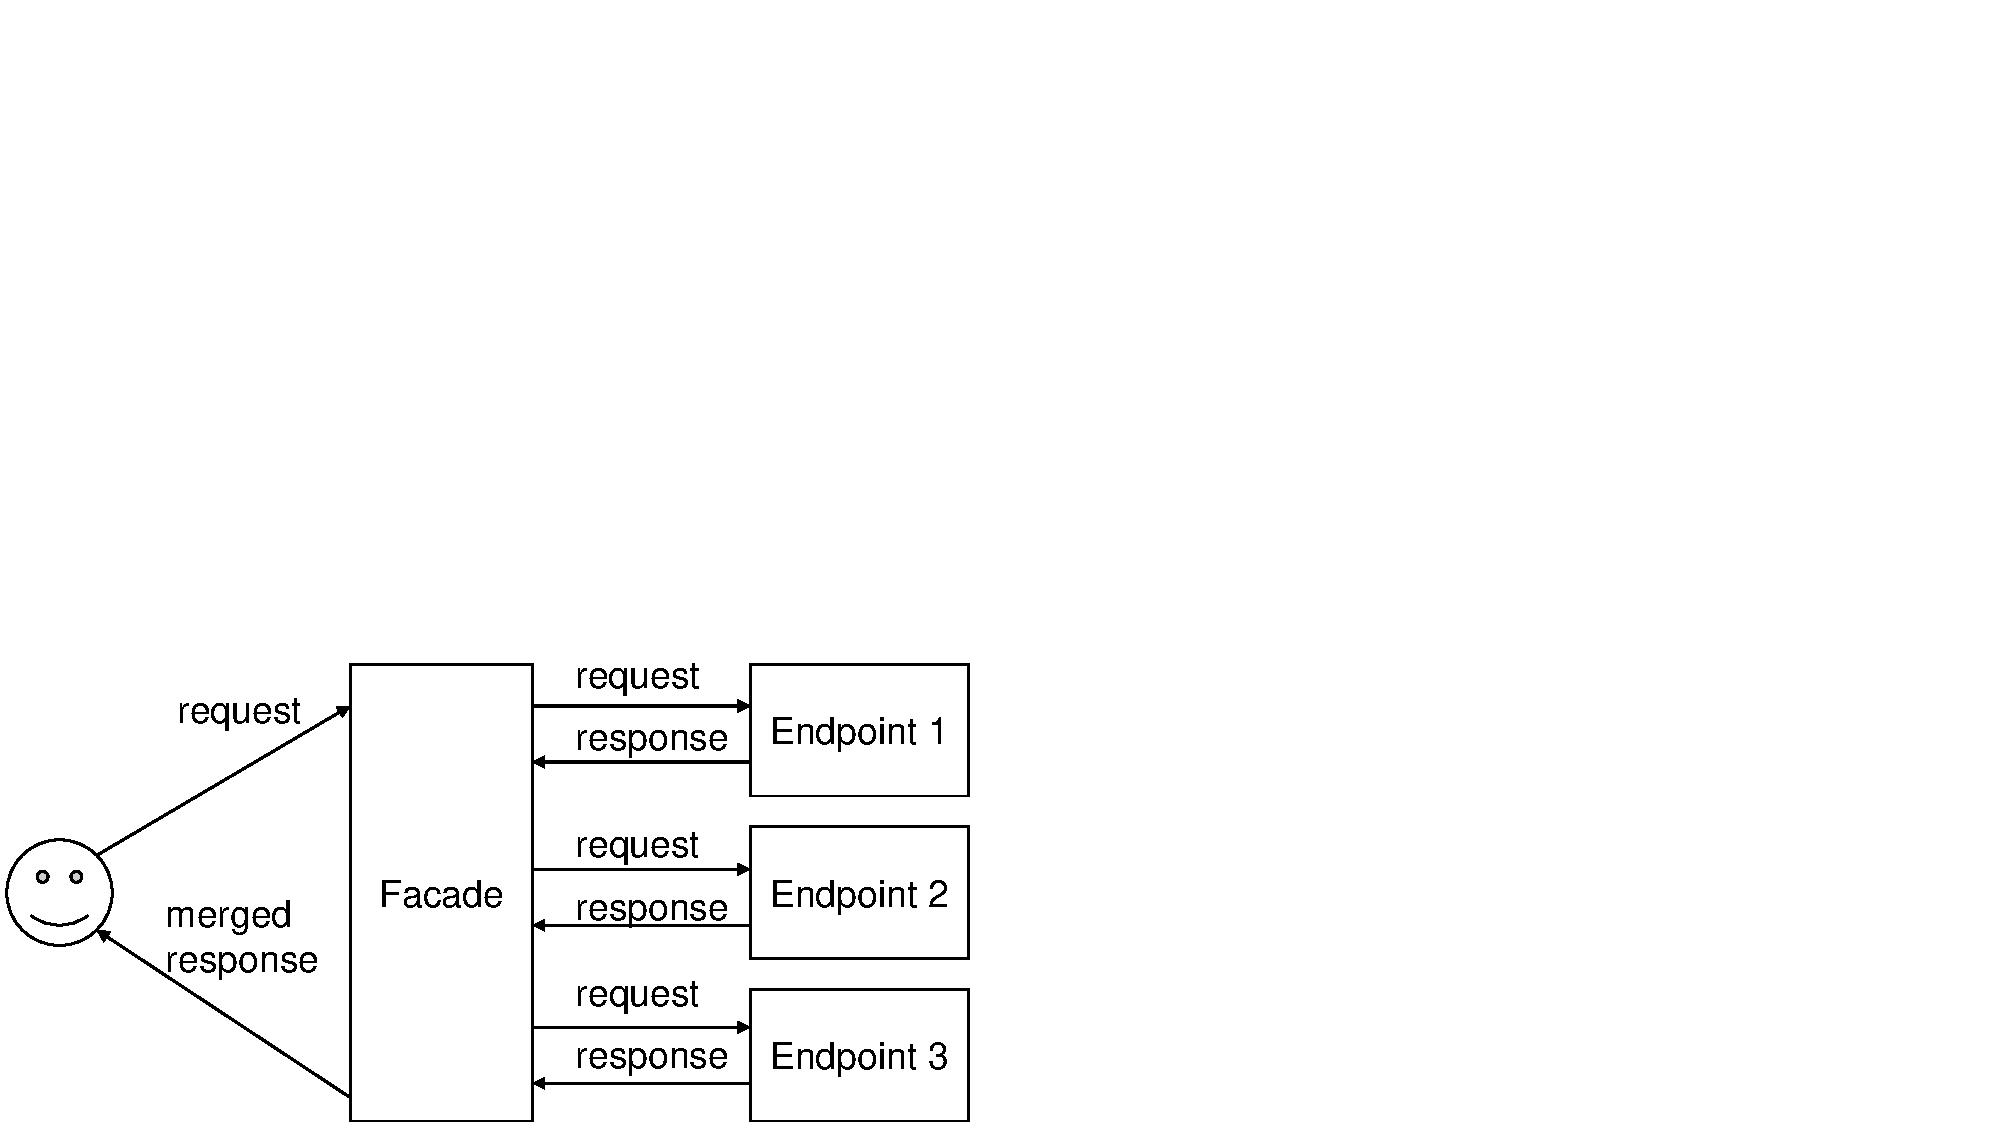
\includegraphics[width=.5\columnwidth,bb=0 0 466 229,clip]{figs1.pdf}
\caption[Overview of the proposed facade]{The user sends a request to the facade; this request is propagated to the relevant \glsacpl{api}. Responses are merged by the facade and returned back to the user.}\label{icwe2019:fig:facade}
\end{figure}

Although the model introduces more time and cost overhead, both can be mitigated by caching results. On the other hand, the facade pattern provides the following benefits:

\begin{itemize}
\item \textbf{Easy to modify:} It requires only small modifications to applications, e.g., changing each concrete endpoint URL.
\item \textbf{Easy to customise:} It merges results from disparate and concrete \glsacpl{api} according to the user's preference.
\item \textbf{Improves reliability:} It enhances reliability of the overall returned result by merging results from different endpoints.
\end{itemize}

\subsection{Merge Operations}\label{icwe2019:sec:merge-operations}

The \glsac{api} facade is applicable to many use cases.
However, this paper focuses on \glsacpl{api} that output a list of labels and scores, as is the case for \glspl{cvs}.
Merge operations involve the mapping of multiple lists and associated scores, produced by multiple \glsacpl{api}, to just one list.
For instance, a \gls{cvs} receives a bowl of fruit as the input image and outputs the following:

\begin{center}
  \texttt{[[`apple', 0.9], [`banana', 0.8]]}
\end{center}

\noindent
where the first item is the label and the second item is the score. Similarly, another computer vision \glsac{api} outputs the following for the same image:

\begin{center}
  \texttt{[[`apple', 0.7], [`cherry', 0.8]]}.  
\end{center}

\noindent
Merge operations can, therefore, merge these two responses into just one response. Naive ways of merging results could make use of \textit{max}, \textit{min}, and \textit{average} operations on the confidence scores. For example, \textit{max} merges results to:

\begin{center}
  \texttt{[[`apple', 0.9], [`banana', 0.8], [`cherry', 0.8]]};
\end{center}

\noindent
\textit{min} merges results to:

\begin{center}
\texttt{[[`apple', 0.7]]}; 
\end{center}

\noindent
and \textit{average} merges results to:

\begin{center}
\texttt{[[`apple', 0.8], [`banana', 0.4], [`cherry', 0.4]]}.
\end{center}

\noindent
However, as the object's labels in each result are natural language, the operations do not exploit the label's semantics when conducting label merging. To improve the quality of the merged results, we consider the ontologies of these labels, as we describe below.

\subsection{Merging Operators for Labels}\label{icwe2019:sec:operator-properties}

Merge operations on labels are $n$-ary operations that map $R^{n}$ to $R$, where $R_i=\{(l_{ij}, s_{ij})\}$ is a response from endpoint $i$ and contains pairs of labels ($l_{ij}$) and scores ($s_{ij}$).
Merge operations on labels have the following properties:
 
\begin{itemize}
\item
\textit{identity} defines that merging a single response should output same response (i.e., $R=\mathrm{merge}(R)$ is always true);
\item
\textit{commutativity} defines that the order of operands should not change the result (i.e., $\mathrm{merge}(R_1, R_2) = \mathrm{merge}(R_2, R_1)$ is always true);
\item
\textit{reflexivity} defines that merging multiple same responses should output same response (i.e., $R=\mathrm{merge}(R, R)$ is always true); and,
\item
\textit{additivity} defines that, for a specific label, the merged response should have higher or equal score for the label if a concrete endpoint has a higher score. Let $R=\mathrm{merge}(R_1, R_2)$ and $R'=\mathrm{merge}(R'_1, R_2)$ be merged responses.
$R_1$ and $R'_1$ are same, except $R'_1$ has a higher score for label $l_x$ than $R_1$. The additive score property requires that $R'$ score for $l_x$ should be greater than or equal to $R$ score for $l_x$.
\end{itemize}

The \textit{max}, \textit{min}, and \textit{average} operations in \cref{icwe2019:sec:merge-operations} follow each of these rules as all operations calculate the score by applying these operations on each score.

\section{Graph of Labels}\label{icwe2019:sec:graph-of-labels}

\Glspl{cvs} typically return lists of labels and their associated scores. In most cases, the label can be a singular word (e.g., `husky') or multiple words (e.g., `dog breed'). Lexical databases, such as WordNet \citep{WordNetMiller1995}, can therefore be used to describe the ontology behind these labels' meanings.
\Cref{icwe2019:fig:labels-graph} is an example of a graph of labels and synsets.
A synset is a grouped set of synonyms for a word.
In this image, we consider two fictional endpoints, endpoints 1--2. We label red nodes as labels from endpoint 1, yellow nodes as labels from endpoint 2, and blue nodes as synsets for the associated labels from both endpoints.
As actual graphs are usually more complex, \cref{icwe2019:fig:labels-graph} is a simplified graph to illustrate the usage of associating labels from two concrete sources to synsets.

\begin{figure}
\centering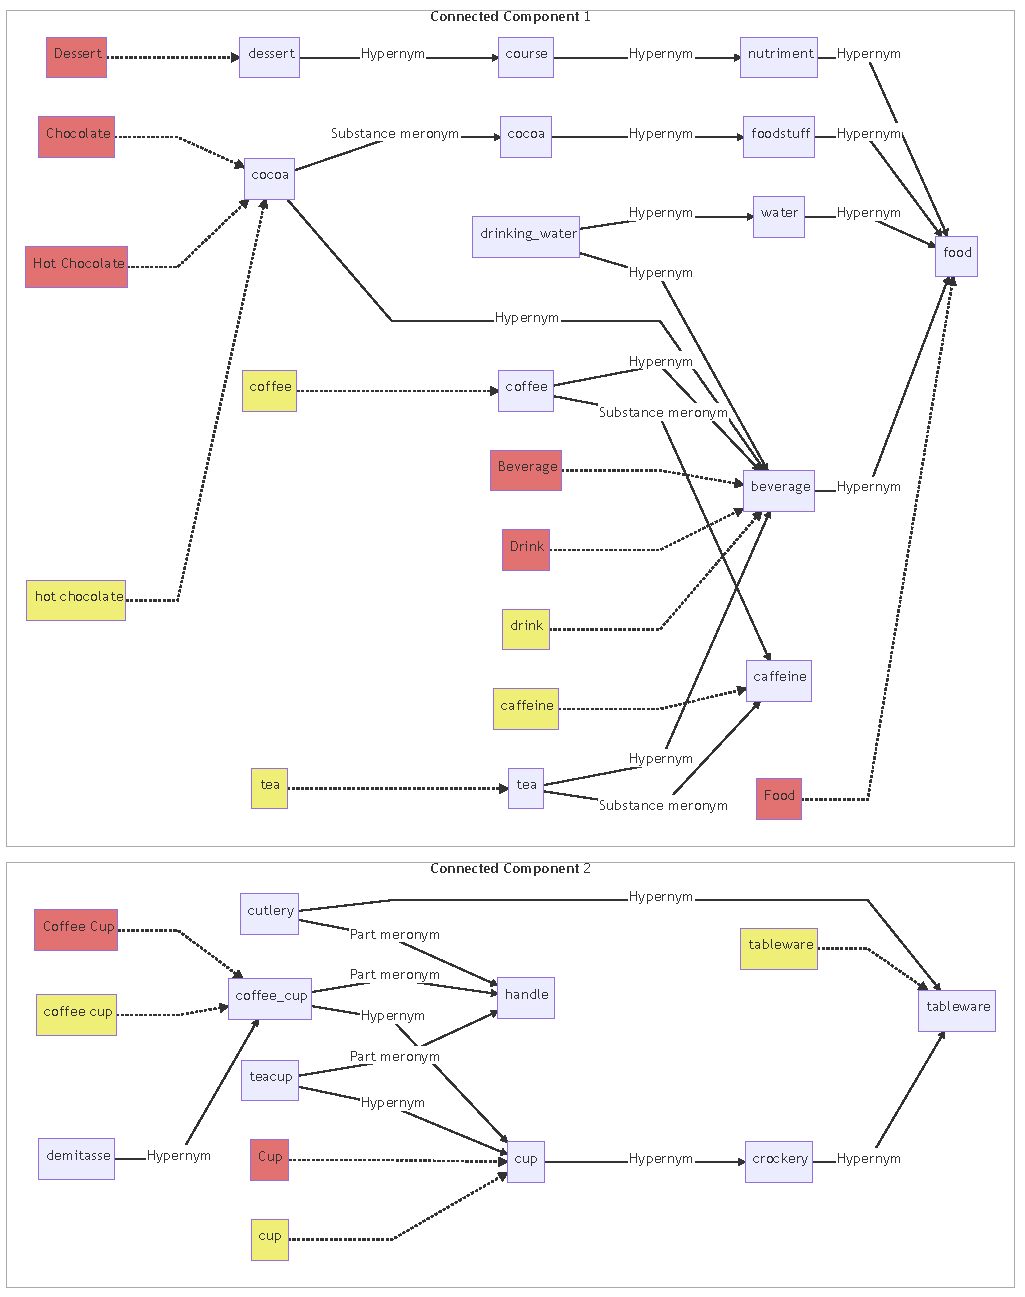
\includegraphics[width=\linewidth]{mermaid_coffee}
\caption[Graph of associated synsets against two different endpoints]{Graph of labels from two concrete endpoints (red and yellow) and their associated synsets related to both words (blue).}\label{icwe2019:fig:labels-graph}
\end{figure}

\subsection{Labels and synsets}\label{icwe2019:sec:label-synsets}

The number of labels depends on input images and concrete \glsac{api} endpoints used.
\Cref{icwe2019:tab:label-count,icwe2019:fig:label-count1} show how many labels are returned, on average per image, from Google Cloud Vision \citepweb{GoogleCloud:Home}, Amazon Rekogition \citepweb{AWS:Home} and Azure Computer Vision \citepweb{Azure:Home} image recognition \glsacpl{api}. These statistics were calculated using 1,000 images from Open Images Dataset V4 \citepweb{OpenImag40:online} Image-Level Labels set.

\begin{table}
\caption[Statistics for the number of labels]{Statistics for the number of labels, on average, per service identified.}\label{icwe2019:tab:label-count}
\centering
\tablefit{\begin{tabular}{l|rrr}
\toprule
\textbf{Endpoint} & \textbf{Average number of labels} & \textbf{Has synset} & \textbf{No synset} \\
\midrule
Amazon Rekognition & $11.42 \pm 7.52$ & $10.74 \pm 7.10$ (94.0\%) & $0.66 \pm 0.87$ \\
Google Cloud Vision & $8.77 \pm 2.15$ & $6.36 \pm 2.22$ (72.5\%) & $2.41 \pm 1.93$ \\
Azure Computer Vision & $5.39 \pm 3.29$ & $5.26 \pm 3.32$ (97.6\%) & $0.14 \pm 0.37$ \\
\bottomrule
\end{tabular}}
\end{table}

\begin{figure}
\centering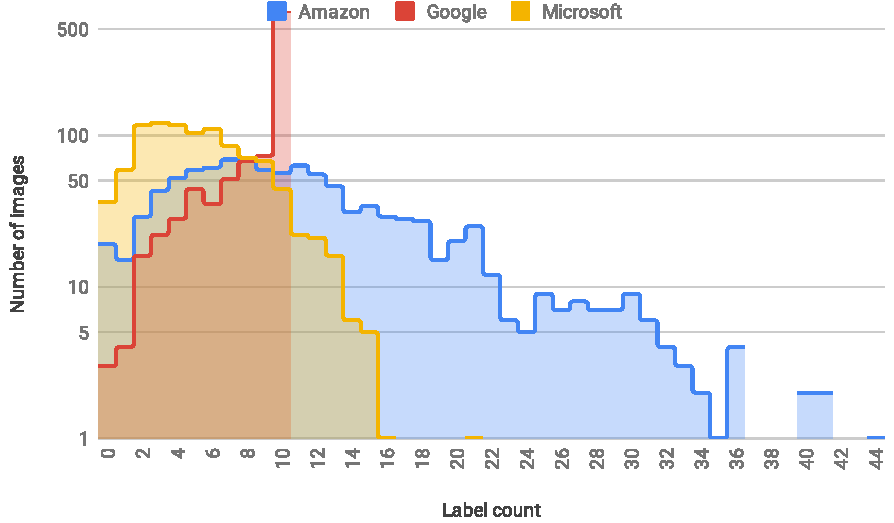
\includegraphics[width=.9\linewidth]{label_count1}
\caption[Label counts per \glsac{api} assessed]{Number of labels responded from our input dataset to three concrete \glsacpl{api} assessed.}
\label{icwe2019:fig:label-count1}
\end{figure}

Labels from Amazon and Microsoft tend to have corresponding synsets, and therefore these endpoints return common words that are found in WordNet.
On the other hand, Google's labels have less corresponding synsets: for example, labels without corresponding synsets are car models and dog breeds.\footnote{We noticed from our upload of 1,000 images that Google tries to identify objects in greater detail.}

\subsection{Connected Components}

A \gls{cc} is a subgraph in which there are paths between any two nodes.
In graphs of labels and synsets, \glspl{cc} are clusters of labels and synsets with similar semantic meaning.
For instance, there are two \glspl{cc} in \cref{icwe2019:fig:labels-graph}.
\gls{cc}~1 in \cref{icwe2019:fig:labels-graph} has \texttt{`beverage'}, \texttt{`dessert'}, \texttt{`chocolate'}, \texttt{`hot chocolate'}, \texttt{`drink'}, and \texttt{`food'} labels from the red first endpoint and \texttt{`coffee'}, \texttt{`hot chocolate'}, \texttt{`drink'}, \texttt{`caffeine'}, and \texttt{`tea'} labels from the yellow second endpoint.
Therefore, these labels are related to \texttt{`drink'}.
On the other hand, \gls{cc}~2 in \cref{icwe2019:fig:labels-graph} has \texttt{`cup'} and \texttt{`coffee cup'} labels from the first red endpoint and \texttt{`cup'}, \texttt{`coffee cup'}, and \texttt{`tableware'} labels from the yellow second endpoint.
These labels are, therefore, related to \texttt{`cup'}.

\begin{figure}
\centering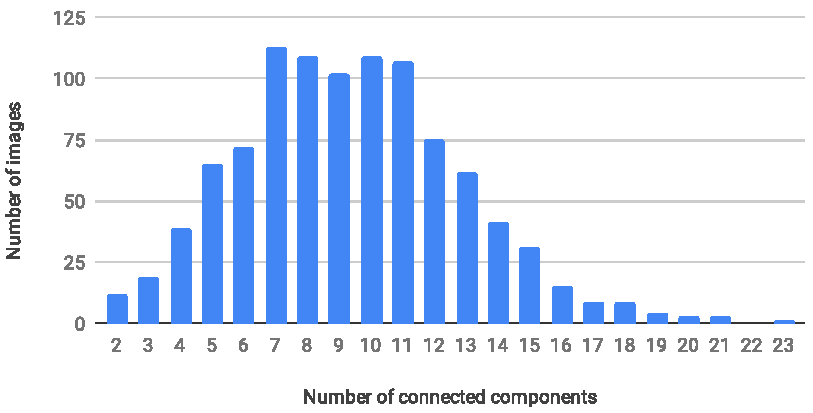
\includegraphics[width=.95\linewidth]{connected_components}
\caption[Connected components vs. images]{Number of connected components compared to the number of images.}\label{icwe2019:fig:connected-components}
\end{figure}

\Cref{icwe2019:fig:connected-components} shows a distribution of number of \glspl{cc} for the 1,000-image label detections on Amazon Rekognition, Google Cloud Vision, and Azure Computer Vision \glsacpl{api}.
The average number of \glspl{cc} is $9.36 \pm 3.49$.
The smaller number of \glspl{cc} means that most of labels have similar meanings, while a larger value means that the labels are more disparate.

\section{API Results Merging Algorithm}\label{icwe2019:sec:algorithm}

Our proposed algorithm to merge labels consists of four parts: (1) mapping labels to synsets, (2) deciding the total number of labels, (3) allocating the number of labels to \glspl{cc}, and (4) selecting labels from \glspl{cc}.

\subsection{Mapping Labels to Synsets}\label{icwe2019:sec:label-to-synset}

Labels returned in \gls{cvs} responses are words (in natural language) that do not always identify their intended meanings.
For instance, a label \textit{orange} may represent the fruit, the colour, or the name of the longest river in South Africa.
To identify the actual meanings behind a label, our facade enumerates all synsets corresponding to labels.
It then finds the most likely synsets for labels by traversing WordNet links.
For instance, if an \glsac{api} endpoint outputs the \texttt{`orange'} and \texttt{`lemon'} labels, the facade regards \texttt{`orange'} as a related synset word of \texttt{`fruit'}.
If an \glsac{api} endpoint outputs \texttt{`orange'} and \texttt{`water'} labels, the facade regards \texttt{`orange'} as a \texttt{`river'}.

\subsection{Deciding Total Number of Labels}\label{icwe2019:sec:allocation-total}

The number of labels in responses from endpoints vary as described in \cref{icwe2019:sec:label-synsets}.
The facade decides the number of merged labels using the numbers of labels from each endpoint.
We formulate the following equation to calculate the number of labels:

\begin{equation*}
\min_i(|R_i|) \leq \frac{\Sigma_i |R_i|}{n} \leq \max_i(|R_i|) \leq \Sigma_i |R_i|
\end{equation*}

\noindent
where $|R|$ is number of labels and scores in response, and $n$ is number of endpoints.
In case of naive operations in \cref{icwe2019:sec:merge-operations}, the following is true:

\begin{align*}
&|\mathrm{merge}_\mathrm{max}(R_1, \ldots, R_n)| \leq \min_i(|R_i|) \\
\max_i(|R_i|) \leq &|\mathrm{merge}_\mathrm{min}(R_1, \ldots, R_n)| \leq \Sigma_i |R_i| \\
\max_i(|R_i|) \leq &|\mathrm{merge}_\mathrm{average}(R_1, \ldots, R_n)| \leq \Sigma_i |R_i|.
\end{align*}

\noindent
The proposal uses $\lfloor \Sigma_i |R_i|/n \rfloor$ to conform to the necessary condition described in \cref{icwe2019:sec:allocation-cc}.

\subsection{Allocating Number of Labels to Connected Components}\label{icwe2019:sec:allocation-cc}

The graph of labels and synsets is then divided into several \glspl{cc}.
The facade decides how many labels are allocated for each \gls{cc}.
For example, in \cref{icwe2019:fig:allocation}, there are three \glspl{cc}, where square-shaped nodes are labels in responses from endpoints.
Text within these label nodes describe which endpoint outputs the label and score, for instance, ``L-1a, 0.9'' is label \textit{a} from endpoint \textit{1} with a score \textit{0.9}.
Circle-shaped nodes represent synsets, where the edges between the label and synset nodes indicate the relationships between them.
Edges between synsets are links in WordNet.

\begin{figure}
\centering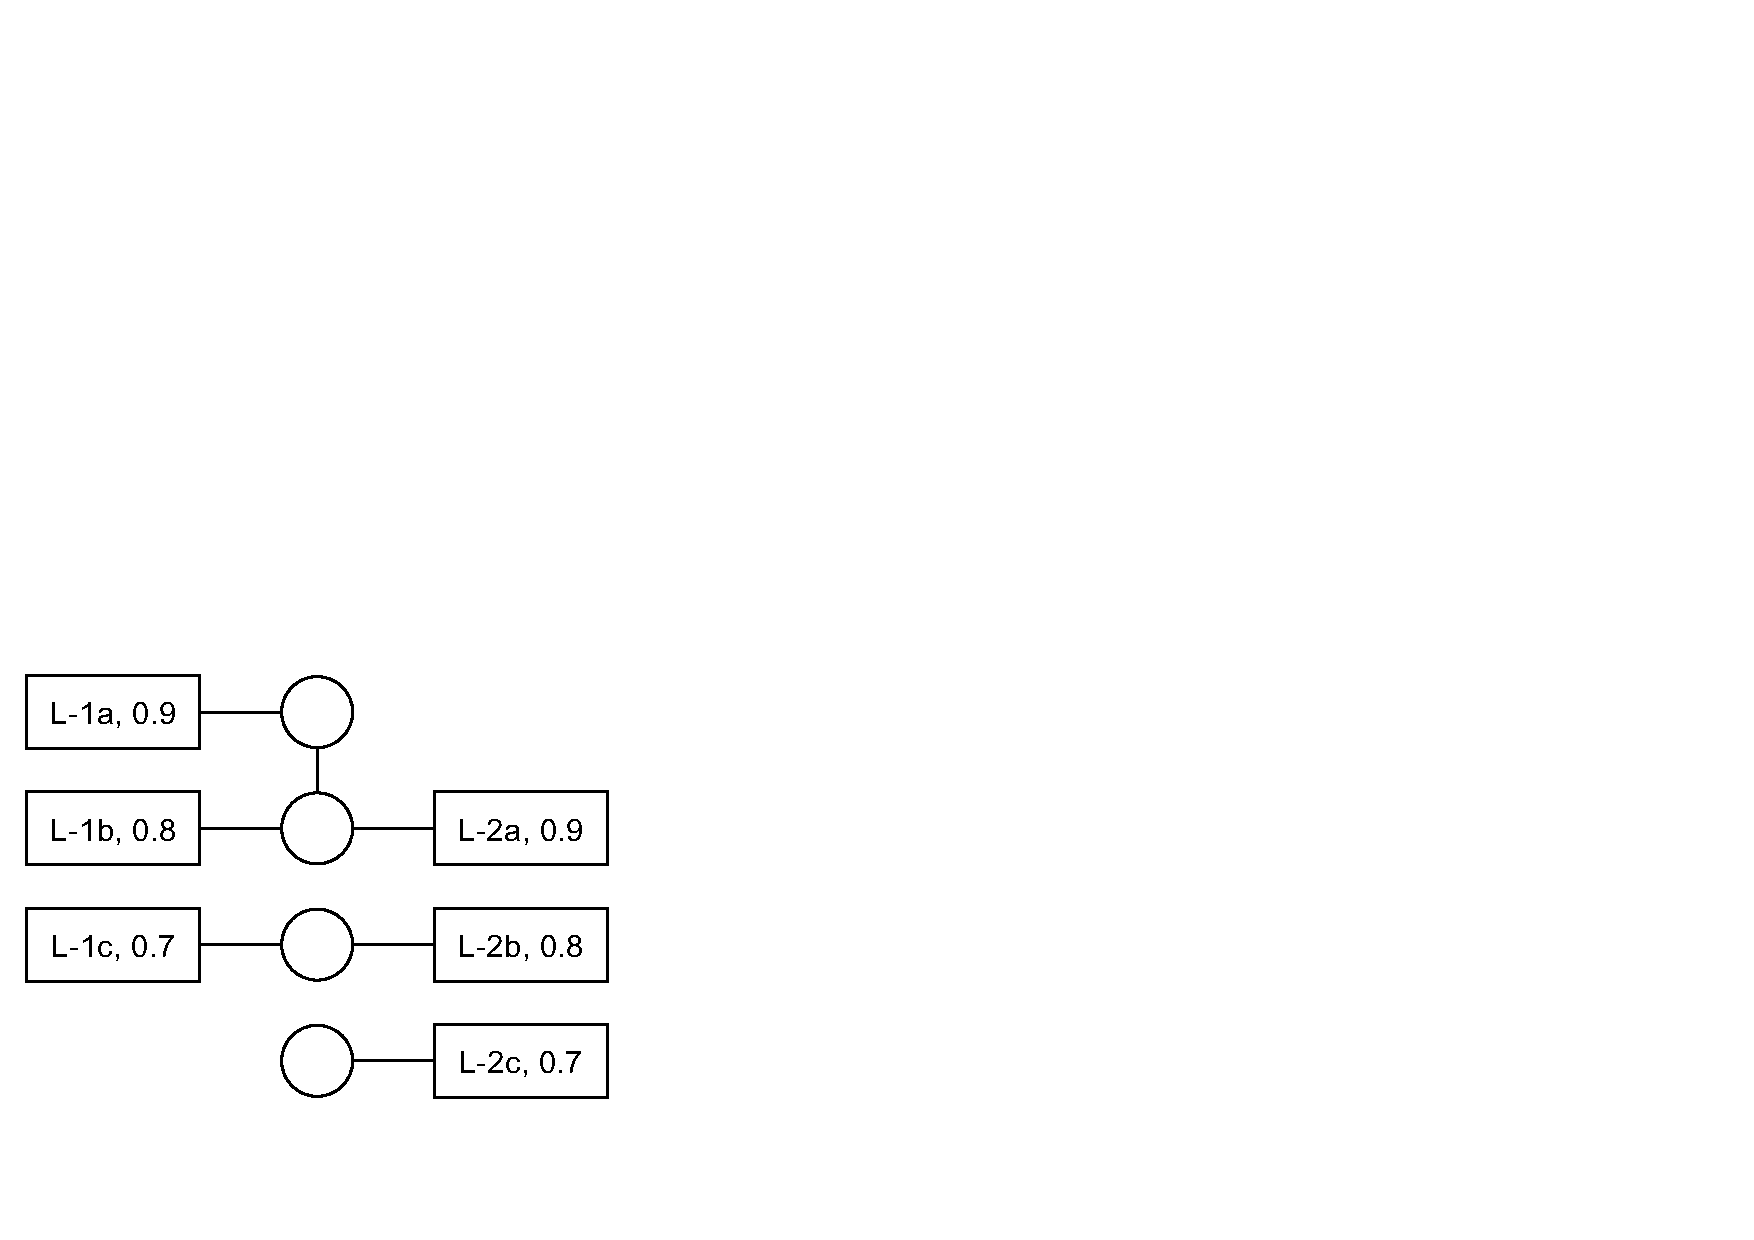
\includegraphics[width=.43\columnwidth,bb=0 0 329 239,clip]{figs2.pdf}
\caption[Allocation to connected components]{Allocation to connected components.}\label{icwe2019:fig:allocation}
\end{figure}

Allegorically, allocating the number of labels to \glspl{cc} is similar to proportional representation in a political voting system, where \glspl{cc} are the political parties and labels are the votes to a party.
Several allocation algorithms are introduced in proportional representation, for instance, the D'Hondt and Hare-Niemeyer methods \citep{Niemeyer2008240}.
However, there are differences from proportional representation in the political context.
For label merging, labels have scores and origin endpoints and such information may improve the allocation algorithm.
For instance, \glspl{cc} supported with more endpoints should have a higher allocation than \glspl{cc} with fewer endpoints, and \glspl{cc} with higher scores should have a higher allocation than \glspl{cc} with lower scores.
We introduce an algorithm to allocate the number of labels to \glspl{cc}. This allocates more to a \gls{cc} with more supporting endpoints and higher scores.
The steps of the algorithm are:

\begin{enumerate}[label=\textbf{Step \Roman*.}, ref={Step \Roman*}, leftmargin=2.75\parindent]
  \item Sort scores separately for each endpoint. \label{icwe2019:li:algorithm-step-sort}
  \item If all \glspl{cc} have an empty score array or more, remove one, and go to \ref{icwe2019:li:algorithm-step-remove-empty}. \label{icwe2019:li:algorithm-step-remove-empty}
  \item Select the highest score for each endpoint and calculate product of highest scores.
  \item A \gls{cc} with the highest product score receives an allocation. This \gls{cc} removes every first element from the score array.
  \item If the requested number of allocations is complete, then stop allocation. Otherwise, go to \ref{icwe2019:li:algorithm-step-remove-empty}. \label{icwe2019:li:algorithm-step-last}
\end{enumerate}

\Cref{icwe2019:tab:allocation1,icwe2019:tab:allocation2,icwe2019:tab:allocation3,icwe2019:tab:allocation4} are examples of allocation iterations.
In \cref{icwe2019:tab:allocation1}, the facade sorts scores separately for each endpoint.
For instance, the first \gls{cc} in \cref{icwe2019:fig:allocation} has scores of 0.9 and 0.8 from endpoint 1 and 0.9 from endpoint 2.
All \glspl{cc} have a non-empty score array or more, so the facade skips \ref{icwe2019:li:algorithm-step-remove-empty}.
The facade then picks the highest scores for each endpoint and \gls{cc}.
\Gls{cc} 1 has the largest product of highest scores and receives an allocation.
In \cref{icwe2019:tab:allocation2}, the first \gls{cc} removes every first score in its array as it received an allocation in \cref{icwe2019:tab:allocation1}.
In this iteration, the second \gls{cc} has largest product of scores and receives an allocation.
In \cref{icwe2019:tab:allocation3}, the second \gls{cc} removes every first score in its array.
At \ref{icwe2019:li:algorithm-step-remove-empty}, all the three \glspl{cc} have an empty array.
The facade removes one empty array from each \gls{cc}.
In \cref{icwe2019:tab:allocation4}, the first \gls{cc} receives an allocation.
The algorithm is applicable if total number of allocation is less than or equal to $\max_i(|R_i|)$ as scores are removed in \ref{icwe2019:li:algorithm-step-remove-empty}.
The condition is a necessary condition.

\begin{table}
\begin{minipage}[b]{.45\linewidth}
\caption[First allocation iteration]{Allocation iteration 1.}\label{icwe2019:tab:allocation1}
\centering
\tablefit{\begin{tabular}{llrr}
\toprule
\textbf{Scores} & \textbf{Highest} & \textbf{Product} & \textbf{Allocated} \\ 
\midrule
\relax [0.9, 0.8], [0.9] & [0.9, 0.9] & 0.81 & 0+1 \\ 
\relax [0.7], [0.8] & [0.7, 0.8] & 0.56 & 0 \\ 
\relax [], [0.7] & [N/A, 0.7] & N/A & 0 \\ 
\bottomrule
\end{tabular}}
\end{minipage}
\hspace{\fill}
\begin{minipage}[b]{.45\linewidth}
\caption[Second allocation iteration]{Allocation iteration 2.}\label{icwe2019:tab:allocation2}
\centering
\tablefit{\begin{tabular}{llrr}
\toprule
\textbf{Scores} & \textbf{Highest} & \textbf{Product} & \textbf{Allocated} \\ 
\midrule
\relax [0.8], [] & [0.8, N/A] & N/A & 1 \\ 
\relax [0.7], [0.8] & [0.7, 0.8] & 0.56 & 0+1 \\ 
\relax [], [0.7] & [N/A, 0.7] & N/A & 0 \\ 
\bottomrule
\end{tabular}}
\end{minipage}

\bigskip

\begin{minipage}[b]{.45\linewidth}
\caption[Third allocation iteration]{Allocation iteration 3.}\label{icwe2019:tab:allocation3}
\centering
\tablefit{\begin{tabular}{llrr}
\toprule
\textbf{Scores} & \textbf{Highest} & \textbf{Product} & \textbf{Allocated} \\ 
\midrule
\relax [0.8], [] &---&---& 1 \\ 
\relax [], [] &---&---& 1 \\ 
\relax [], [0.7] &---&---& 0 \\ 
\bottomrule
\end{tabular}}
\end{minipage}
\hspace{\fill}
\begin{minipage}[b]{.45\linewidth}
\caption[Fourth allocation iteration]{Allocation iteration 4.}\label{icwe2019:tab:allocation4}
\centering
\tablefit{\begin{tabular}{llrr}
\toprule
\textbf{Scores} & \textbf{Highest} & \textbf{Product} & \textbf{Allocated} \\ 
\midrule
\relax [0.8] & [0.8] & 0.8 & 1+1 \\ 
\relax [] & [N/A] & N/A & 1 \\ 
\relax [0.7] & [0.7] & 0.7 & 0 \\ 
\bottomrule
\end{tabular}}
\end{minipage}
\end{table}

\subsection{Selecting Labels from Connected Components}\label{icwe2019:sec:select-highest}

For each \gls{cc}, the facade applies the \textit{average} operator from \cref{icwe2019:sec:merge-operations} and takes labels with $n$-highest scores up to allocation, as per \cref{icwe2019:sec:allocation-cc}.

\subsection{Conformance to properties}

\Cref{icwe2019:sec:operator-properties} defines four properties: identity, commutativity, reflexivity, and additivity.
Our proposed method conforms to these properties:

\begin{itemize}
  \item \textit{identity:} the method outputs same result if there is one response;
  \item \textit{commutativity:} the method does not care about ordering of operands;
  \item \textit{reflexivity:} the allocations to \glspl{cc} are same to number of labels in \glspl{cc}; and
  \item \textit{additivity:} increases in score increases or does not change the allocation to the corresponding \gls{cc}.
\end{itemize}

\section{Evaluation}\label{icwe2019:sec:evaluation}

\subsection{Evaluation Method}\label{icwe2019:sec:evaluation-method}

To evaluate the merge methods, we merged \gls{cvs} results from three representative image analysis \glsac{api} endpoints and compared these merged results against human-verified labels.
Images and human-verified labels are sourced from 1,000 randomly-sampled images from the Open Images Dataset V4 \citepweb{OpenImag40:online} Image-Level Labels test set.

The first three rows in \cref{icwe2019:tab:evaluation} are the evaluation of original responses from each \glsac{api} endpoint.
Precision, recall, and F-measure in \cref{icwe2019:tab:evaluation} do not reflect actual values: for instance, it appears that Google performs best at first glance, but this is mainly because Google's labels are similar to that of the Open Images label set.

The Open Images Dataset uses 19,995 classes for labelling. The human-verified labels for the 1,000 images contain 8,878 of these classes.
\Cref{icwe2019:tab:label-match} shows the correspondence between each service's labels and the Open Images Dataset classes.
For instance, Amazon Rekognition outputs 11,416 labels in total for 1,000 images.
There are 1,409 unique labels in 11,416 labels.
1,111 labels out of 1,409 can be found in Open Images Dataset classes.
Rekognition's labels matches to Open Images Dataset classes at 78.9\% ratio, while Google has an outstanding matched percentage of 94.1\%.
This high match is likely due to Google providing both Google Cloud Vision and the Open Images Dataset---it is likely that they are trained on the same data and labels.
An endpoint with higher matched percentage has a more similar label set to the Open Images Dataset classes.
However, a higher matched percentage does not mean imply \textit{better quality} of an \glsac{api} endpoint; it will increase apparent precision, recall, and F-measure only.

The true and false positive (TP/FP) label averages and the TP/FP ratio is shown in \cref{icwe2019:tab:evaluation}.
Where the TP/FP ratio is larger, the scores are more reliable, however it is possible to increase the TP/FP ratio by adding more false labels with low scores.
On the other hand, it is impossible to increase F-measure intentionally, because increasing precision will decrease recall, and vice versa.
Hence, the importance of the F-measure statistic is critical for our analysis.

Let $R_A$, $R_G$, and $R_M$ be responses from Amazon Rekognition, Google Cloud Vision, and Microsoft's Azure Computer Vision, respectively.
There are four sets of operands, i.e., $(R_A, R_G)$, $(R_G, R_M)$, $(R_M, R_A)$, and $(R_A, R_G, R_M)$.
\Cref{icwe2019:tab:evaluation} shows the evaluation of each operands set, \cref{icwe2019:tab:evaluation-average} shows the averages of the four operands sets, and \cref{icwe2019:fig:fmeasure-comparison} shows the comparison of F-measure for each methods.

\begin{table}
\caption[Matching to human-verified labels]{Matching to human-verified labels.}\label{icwe2019:tab:label-match}
\centering
\begin{tabular}{l|rrrr}
\toprule
\textbf{Endpoint} & \textbf{Total} & \textbf{Unique} & \textbf{Matched} & \textbf{Matched} \% \\
\midrule
Amazon Rekognition & 11,416 & 1,409 & 1,111 & 78.9 \\
Google Cloud Vision & 8,766 & 2,644 & 2,487 & 94.1 \\
Azure Computer Vision & 5,392 & 746 & 470 & 63.0 \\
\bottomrule
\end{tabular}

\bigskip

\caption[Evaluation results of the facade]{Evaluation results. A = Amazon Rekognition, G = Google Cloud Vision, M = Microsoft's Azure Computer Vision.}\label{icwe2019:tab:evaluation}
\centering
\tablefit{\begin{tabular}{ll|rrr|rrr}

\toprule
\textbf{Operands} & \textbf{Operator} & \textbf{Precision} & \textbf{Recall} & \textbf{F-measure} & \textbf{TP average} & \textbf{FP average} & \textbf{TP/FP ratio} \\
\midrule

A & & 0.217 & 0.282 & 0.246 & $0.848 \pm 0.165$ & $0.695 \pm 0.185$ & 1.220 \\
G & & 0.474 & 0.465 & 0.469 & $0.834 \pm 0.121$ & $0.741 \pm 0.132$ & 1.126 \\
M & & 0.263 & 0.164 & 0.202 & $0.858 \pm 0.217$ & $0.716 \pm 0.306$ & 1.198 \\

A, G & Min & 0.771 & 0.194 & 0.310 & $0.805 \pm 0.142$ & $0.673 \pm 0.141$ & 1.197 \\
A, G & Max & 0.280 & 0.572 & 0.376 & $0.850 \pm 0.136$ & $0.712 \pm 0.171$ & 1.193 \\
A, G & Average & 0.280 & 0.572 & 0.376 & $0.546 \pm 0.225$ & $0.368 \pm 0.114$ & 1.485 \\
A, G & D'Hondt & 0.350 & 0.389 & 0.369 & $0.713 \pm 0.249$ & $0.518 \pm 0.202$ & 1.377 \\
A, G & Hare-Niemeyer& 0.344 & 0.384 & 0.363 & $0.723 \pm 0.242$ & $0.527 \pm 0.199$ & 1.371 \\
A, G & Proposal & 0.380 & 0.423 & 0.401 & $0.706 \pm 0.239$ & $0.559 \pm 0.190$ & 1.262 \\

G, M & Min & 0.789 & 0.142 & 0.240 & $0.794 \pm 0.209$ & $0.726 \pm 0.210$ & 1.093 \\
G, M & Max & 0.357 & 0.521 & 0.424 & $0.749 \pm 0.135$ & $0.729 \pm 0.231$ & 1.165 \\
G, M & Average & 0.357 & 0.521 & 0.424 & $0.504 \pm 0.201$ & $0.375 \pm 0.141$ & 1.342 \\
G, M & D'Hondt & 0.444 & 0.344 & 0.388 & $0.696 \pm 0.250$ & $0.551 \pm 0.254$ & 1.262 \\
G, M & Hare-Niemeyer & 0.477 & 0.375 & 0.420 & $0.696 \pm 0.242$ & $0.591 \pm 0.226$ & 1.179 \\
G, M & Proposal & 0.414 & 0.424 & 0.419 & $0.682 \pm 0.238$ & $0.597 \pm 0.209$ & 1.143 \\

M, A & Min & 0.693 & 0.143 & 0.237 & $0.822 \pm 0.201$ & $0.664 \pm 0.242$ & 1.239 \\
M, A & Max & 0.185 & 0.318 & 0.234 & $0.863 \pm 0.178$ & $0.703 \pm 0.229$ & 1.228 \\
M, A & Average & 0.185 & 0.318 & 0.234 & $0.589 \pm 0.262$ & $0.364 \pm 0.144$ & 1.616 \\
M, A & D'Hondt & 0.271 & 0.254 & 0.262 & $0.737 \pm 0.261$ & $0.527 \pm 0.223$ & 1.397 \\
M, A & Hare-Niemeyer & 0.260 & 0.245 & 0.253 & $0.755 \pm 0.251$ & $0.538 \pm 0.218$ & 1.402 \\
M, A & Proposal & 0.257 & 0.242 & 0.250 & $0.769 \pm 0.244$ & $0.571 \pm 0.205$ & 1.337 \\

A, G, M & Min & 0.866 & 0.126 & 0.220 & $0.774 \pm 0.196$ & $0.644 \pm 0.219$ & 1.202 \\
A, G, M & Max & 0.241 & 0.587 & 0.342 & $0.857 \pm 0.142$ & $0.714 \pm 0.210$ & 1.201 \\
A, G, M & Average & 0.241 & 0.587 & 0.342 & $0.432 \pm 0.233$ & $0.253 \pm 0.106$ & 1.712 \\
A, G, M & D'Hondt & 0.375 & 0.352 & 0.363 & $0.678 \pm 0.266$ & $0.455 \pm 0.208$ & 1.492 \\
A, G, M & Hare-Niemeyer & 0.362 & 0.340 & 0.351 & $0.693 \pm 0.260$ & $0.444 \pm 0.216$ & 1.559 \\
A, G, M & Proposal & 0.380 & 0.357 & 0.368 & $0.684 \pm 0.259$ & $0.484 \pm 0.200$ & 1.414 \\

\bottomrule
\end{tabular}}

\bigskip

\caption[Average of evaluation result of the facade]{Average of the evaluation result.}\label{icwe2019:tab:evaluation-average}
\centering
\begin{tabular}{l|rrr|r}
\toprule
\textbf{Operator} & \textbf{Precision} & \textbf{Recall} & \textbf{F-measure} & \textbf{TP/FP ratio} \\
\midrule
Min & 0.780 & 0.151 & 0.252 & 1.183 \\
Max & 0.266 & 0.500 & 0.344 & 1.197 \\
Average & 0.266 & 0.500 & 0.344 & 1.539 \\
D'Hondt & 0.361 & 0.335 & 0.346 & 1.382 \\
Hare-Niemeyer & 0.361 & 0.336 & 0.347 & 1.378 \\
Proposal & 0.358 & 0.362 & 0.360 & 1.289 \\
\bottomrule
\end{tabular}
\end{table}

\begin{figure}
\centering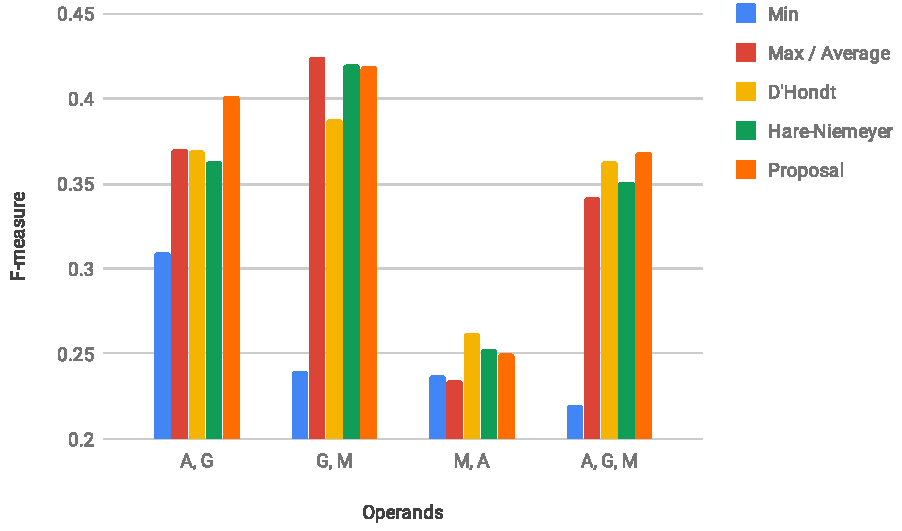
\includegraphics[width=.76\columnwidth]{fmeasures}
\caption[F-measure comparison]{F-measure comparison.}\label{icwe2019:fig:fmeasure-comparison}
\end{figure}

\subsection{Naive Operators}

Results of \textit{min}, \textit{max}, and \textit{average} operators are shown in \cref{icwe2019:tab:evaluation,icwe2019:tab:evaluation-average,icwe2019:fig:fmeasure-comparison}.
The \textit{min} operator is similar to \textit{union} operator of set operation, and outputs all labels of operands.
The precision of the \textit{min} operator is always greater than any precision of operands, and the recall is always lesser than any precision of operands.
\textit{Max} and \textit{average} operators are similar to \textit{intersection} operator of set operations.
Both operators output intersection of labels of operands and there is no clear relation to the precision and recall of operands.
Since both operators have the same precision, recall, and F-measure, \cref{icwe2019:fig:fmeasure-comparison} groups them into one.
The \textit{average} operator performs well on the TP/FP ratio, where most of the same labels from multiple endpoints are TPs.
In many cases of the four operand sets, all naive operators' F-measures are between F-measures of operands.
None of naive operators therefore improve results by merging responses from multiple endpoints.

\subsection{Traditional Proportional Representation Operators}

There are many existing allocation algorithms in proportional representation, e.g., the \citeauthor{Niemeyer2008240} method \citep{Niemeyer2008240}.
These methods may be replacements of those in \cref{icwe2019:sec:allocation-cc}.
Other steps, i.e., \cref{icwe2019:sec:label-to-synset,icwe2019:sec:allocation-total,icwe2019:sec:select-highest}, are the same as for our proposed technique.
\Cref{icwe2019:tab:evaluation,icwe2019:tab:evaluation-average,icwe2019:fig:fmeasure-comparison} show the result of these traditional proportional representation algorithms.
Averages of F-measures by traditional proportional representation operators are almost equal to that of the \textit{max} and \textit{average} operators.
It is worth noting that merging $M$ and $A$ responses results in a better F-measure than each F-measure of $M$ and $A$ individually.
As these are not biased to human-verified labels, situations in the real-world usage should, therefore, be similar to the case of $M$ and $A$.
Hence, RQ1 is true.

\subsection{New Proposed Label Merge Technique}

As shown in \cref{icwe2019:tab:evaluation-average}, our proposed new method performs best in F-measure.
Instead, the TP/FP ratio is less than \textit{average}, the D'Hondt method, and Hare-Niemeyer method.
As described in \cref{icwe2019:sec:evaluation-method}, we argue that F-measure is a more important measure than the TP/FP ratio (in this case).
Therefore, RQ2 is true.
Shown in \cref{icwe2019:tab:evaluation}, our proposed new method improves the results when merging $M$ and $A$ in non-biased endpoints.
It is similar to traditional proportional representation operators, but does not perform as well.
However, it performs better on other operand sets, and performs best overall as shown in \cref{icwe2019:fig:fmeasure-comparison}.

\subsection{Performance}

We used AWS EC2 m5.large instance (2 vCPUs, 2.5 GHz Intel Xeon, 8 GiB RAM); Amazon Linux 2 AMI (HVM), SSD Volume Type; Node.js 8.12.0. It takes 0.370 seconds to merge responses from three endpoints.
Computational complexity of the algorithm in \cref{icwe2019:sec:allocation-cc} is $O(n^2)$, where $n$ is total number of labels in responses.
(The estimation assumes that the number of endpoints is a constant.)
Complexity of \ref{icwe2019:li:algorithm-step-sort} in \cref{icwe2019:sec:allocation-cc} is $O(n \log n)$, as the worst case is that all $n$ labels are from one single endpoint and all $n$ labels are in one \gls{cc}.
Complexity of \ref{icwe2019:li:algorithm-step-remove-empty} to \ref{icwe2019:li:algorithm-step-last} is $O(n^2)$, as the number of \glspl{cc} is less than or equal to $n$ and number of iterations are less than or equal to $n$.
As \cref{icwe2019:tab:label-count} shows, the averaged total number of three endpoints is 25.58.
Most of time for merging is consumed by looking up WordNet synsets (\cref{icwe2019:sec:label-to-synset}). 
The \glsac{api} facade calls each \glsacpl{api} on actual endpoints in parallel.
It takes about 5 seconds, which is much longer than 0.370 seconds taken for the merging of responses.

\section{Conclusions and Future Work}\label{icwe2019:sec:conclusion}

In this paper, we propose a method to merge responses from \glspl{cvs}.
Our method merges \glsac{api} responses better than naive operators and other proportional representation methods (i.e., D'Hondt and Hare-Niemeyer).
The average of F-measure of our method marks 0.360; the next best method, Hare-Niemeyer, marks 0.347.
Our method and other proportional representation methods are able to improve the F-measure from original responses in some cases.
Merging non-biased responses results in an F-measure of 0.250, while original responses have an F-measure between 0.246 and 0.242.
Therefore, users can improve their applications' precision with small modification, i.e., by switching from a singular URL endpoint to a facade-based architecture.
The performance impact by applying facades is small, because overhead in facades is much smaller than \glsac{api} invocation.
Our proposal method conforms identity, commutativity, reflexivity, and additivity properties and these properties are advisable for integrating multiple responses.

Our idea of a proportional representation approach can be applied to other \glspl{iws}.
If the response of such a service is list consisting of an entity and score, and if there is a way to group entities, a proposal algorithm can be applied.
The opposite approach is to improve results by inferring labels.
Our current approach picks some of the labels returned by endpoints.
\Glspl{iws} are not only based on supervised \gls{ml}---thus to cover a wide range of \glspl{iws}, it is necessary to classify and analyse each \glsacpl{api} and establish a method to improve results by merging.
Currently graph structures of labels and synsets (\cref{icwe2019:fig:labels-graph}) are not considered when merging results.
Propagating scores from labels could be used, losing the additivity property but improving results for users.
There are many ways to propagate scores.
For instance, setting propagation factors for each link type would improve merging and could be customised for users' preferences.
It would be possible to generate an \glsac{api} facade automatically.
\glsacpl{api} with the same functionality have same or similar signatures.
Machine-readable \glsac{api} documentation, for instance, Open\glsac{api} Specification, could help a generator to build an \glsac{api} facade.
